\documentclass{beamer}

\usetheme[progressbar=head, block=fill]{metropolis}
\usepackage[utf8]{inputenc}
\usepackage[makeroom]{cancel}
\usepackage{amsmath}

\usepackage{amsmath}
\usepackage{amsfonts}
\usepackage{mathtools}

\usepackage{siunitx} 

\usepackage{manfnt}
\usepackage{graphicx}
\usepackage[dvipsnames]{xcolor}
\definecolor{dgreen}{rgb}{0,0.6,0}
\usepackage{amssymb}
\usepackage{pifont}
\usepackage{mathtools}
\usepackage{multimedia}
\usepackage{media9}
\usepackage{centernot}
\usepackage{amsthm}

\graphicspath{ {figures/} }

\renewcommand{\vec}[1]{\boldsymbol{#1}}
\newcommand{\matr}[1]{\mathbf{#1}}
\newcommand{\cmark}{\ding{51}}%
\newcommand{\xmark}{\ding{55}}%

\newcommand{\unitvec}[1]{\hat{\boldsymbol{#1}}}
\newcommand{\transpose}{^{\mathrm{T}}}

\newcommand{\cubicFrame}[1]{{\color{orange}#1}}
\newcommand{\qx}[1]{{\color{red}#1}}
\newcommand{\qy}[1]{{\color{dgreen}#1}}
\newcommand{\qz}[1]{{\color{blue}#1}}
\newcommand{\theory}[0]{\hfill \color{red}{Theory}}
\newcommand{\cubli}[0]{\hfill \color{dgreen}{Application} 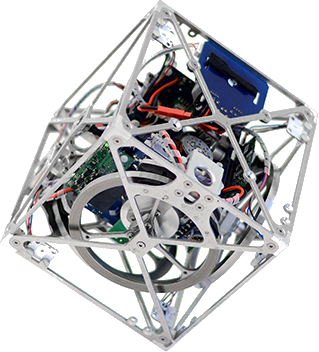
\includegraphics[scale=0.1]{cubli_icon.png}}

\date{17/05/2017}

\title[]{Controllability, observability and Noninteracting control of the Cubli}
\subtitle{Corso di LM in Ingegneria Robotica ed Automazione \\
  Controllo dei Robot}
\author{Students:\hfill Supervisors:\\
Nicola Piga \hfill Prof. Antonio Bicchi\\
Giulio Romualdi \hfill Ing. Manuel Bonilla\\
\hphantom{placeholder}\hfill Ing. Manolo Garabini}
\institute[]{Università di Pisa}
\begin{document}
%\beamertemplatenavigationsymbolsempty

\begin{frame}
  \maketitle
  %% \hskip-in
  %% \centering
  %% \begin{columns}
  %%   \begin{column}{0.4\columnwidth}
  %%   \end{column}
  %%   \begin{column}{0.265\columnwidth}
  %%     \centering
  %%     \includegraphics[width=20mm]{cherubino}
  %%   \end{column}
  %%   \begin{column}{0.6\columnwidth}
  %%     \vskip.1in
  %%     \hskip.3in
  %%     Supervisors:\\
  %%     \hskip.3in
  %%     Prof. Antonio Bicchi\\
  %%     \hskip.3in
  %%     Ing. Manuel Bonilla\\
  %%   \end{column}
  %% \end{columns}
\end{frame}

\section*{Introduction}
In this report the theory of nonlinear systems is applied to a mechanical system known in the literature
as the Cubli \cite{Gajamohan2013}. It is a reaction wheel based 3D inverted pendulum consisting of a $\SI{15}{\centi\meter}$
sided cube with flywheels mounted on three faces.
\begin{figure}[h]
  \centering
  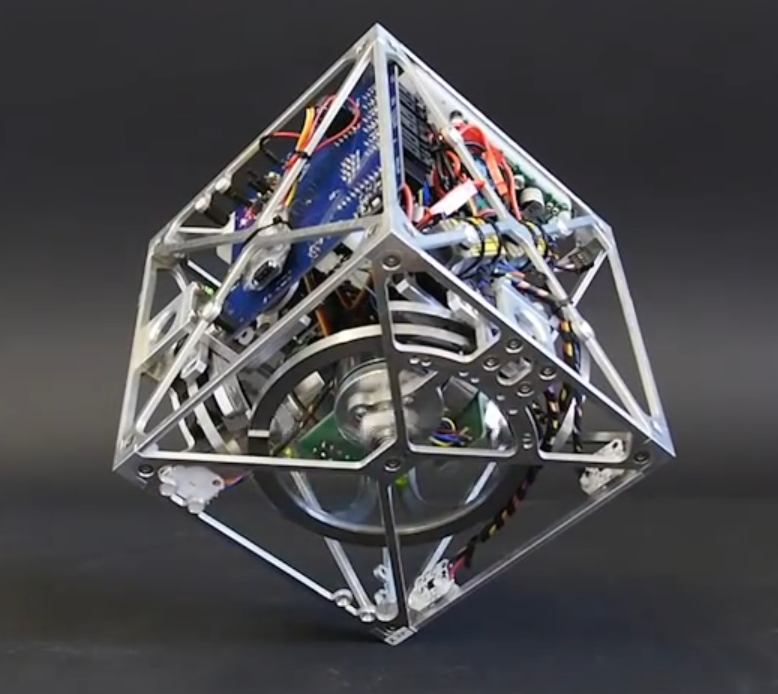
\includegraphics[scale=0.5]{cubli.png}
  \caption{The Cubli}
\end{figure}
\par
In the section one the equations of motion of the system are derived in standard manipulator form and are rewritten
in control affine form which is required to apply the theory of nonlinear systems. Also the equilibria of the system
are described.
\par
In the section two and three the theory regarding nonlinear controllability and observability is briefly recalled
and then is applied to the system.
\par
In the last section a nonlinear controller is developed using the Noninteracting approach, from Isidori, which is
introduced preliminarly. Then the results of the simulation in which the cube perform a pure yaw motion while balancing
on its corner are presented.

\newpage

\section{Equations of motion}
\begin{frame}{Configuration vector}
  \[  
  \vec{q} =
  \begin{bmatrix}
    \theta_{1} & \theta_{2} & \theta_{3} & q_{x} & q_{y} & q_{z}
  \end{bmatrix} \transpose
  \]
  \vskip-0.1in
  \begin{columns}
    \begin{column}{0.55\textwidth}
      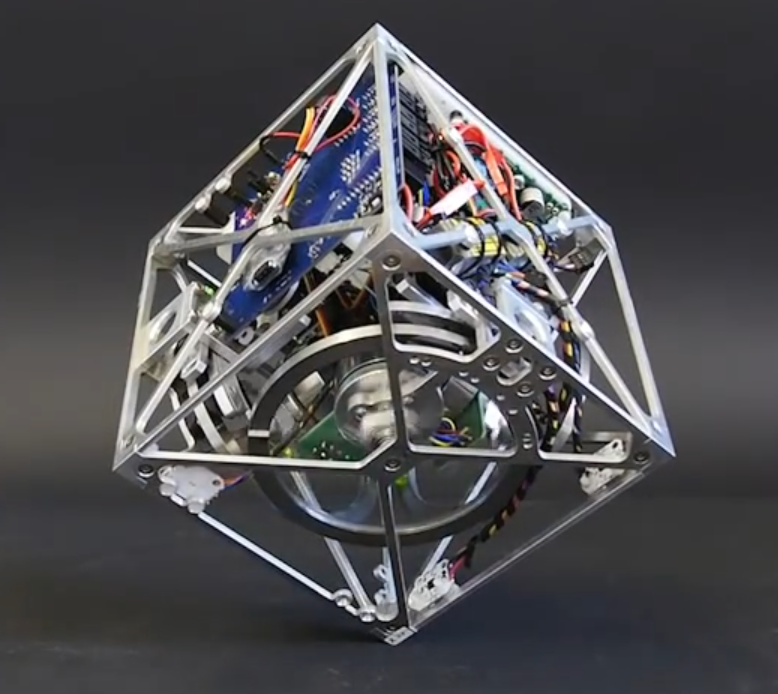
\includegraphics[width=\columnwidth]{cubli}
    \end{column}
    \begin{column}{0.6\textwidth}
      \begin{block}{Attitude}
        \begin{itemize}
        \item[-] Body fixed reference frame $\{C\} = (O_c; \hat{\vec{i}}_c, \hat{\vec{j}}_c, \hat{\vec{k}}_c)$
        \item[-] Inertial reference frame $\{S\} = (O_s; \hat{\vec{i}}_s, \hat{\vec{j}}_s, \hat{\vec{k}}_s)$
        \item[-] $R_{SC}(\vec{\theta}) = R_z(\theta_1)R_y(\theta_2)R_x(\theta_3)$
        \end{itemize}
      \end{block}
      \begin{block}{Flywheels}
        $q_x$, $q_y$ and $q_z$ are the flywheel angular positions
      \end{block}
    \end{column}
  \end{columns}
\end{frame}

\begin{frame}{Notation \footnote[frame]{All quantities expressed in $\{C\}$}}
  \begin{columns}[t]
    \begin{column}{0.5\textwidth}
      \begin{block}{Velocities}
        \begin{itemize}
        \item[-] $\prescript{c}{}{\vec{v}}_{G_{c}}$: cubic frame CoM linear velocity
        \item[-] $\prescript{c}{}{\vec{v}}_{G_{i}}$: i-th flywheel CoM linear velocity
        \item[-] $\prescript{c}{}{\vec{\omega}}_{c}$: cubic frame angular velocity
        \item[-] $\prescript{c}{}{\vec{\omega}}_{i}$: i-th flywheel angular velocity
        \end{itemize}
      \end{block}
    \end{column}
    \begin{column}{0.5\textwidth}
      \begin{block}{Inertial quantities}
        \begin{itemize}
        \item[-] $m_c$: cubic frame mass
        \item[-] $m_i$: i-th flywheels mass
        \item[-] $\prescript{c}{}{\mathfrak{J}}_{G_{c}}$: cubic frame inertia matrix of the 
        \item[-] $\prescript{c}{}{\mathfrak{J}}_{G_{i}}$: i-th flywheel inertia matrix
        \end{itemize}
      \end{block}
    \end{column}
  \end{columns}
\end{frame}

\begin{frame}{Inertia matrices and parameters}
  \begin{columns}
    \begin{column}{0.55\textwidth}
      \begin{block}{Inertia matrices}
        \vskip-0.1in
      \[
  \begin{split}
    &\prescript{c}{}{\mathfrak{J}}_{G_{x}} = 
    \left[
      \begin{smallmatrix}
        \frac{m r^2}{2} & 0 & 0\\
      0 & \frac{m\left(h^2 + 3 r^2 \right)}{12}  & 0\\
      0 & 0 & \frac{m\left(h^2 + 3 r^2 \right)}{12}
      \end{smallmatrix}
      \right]\\
    &\prescript{c}{}{\mathfrak{J}}_{G_{y}} = 
    \left[
    \begin{smallmatrix}
      \frac{m\left(h^2 + 3 r^2 \right)}{12} & 0 & 0\\
      0 & \frac{m r^2}{2} & 0\\
      0 & 0 & \frac{m\left(h^2 + 3 r^2 \right)}{12}
    \end{smallmatrix}
    \right] \\
    &\prescript{c}{}{\mathfrak{J}}_{G_{z}} = 
    \left[
      \begin{smallmatrix}
        \frac{m\left(h^2 + 3 r^2 \right)}{12} & 0 & 0\\
        0 & \frac{m\left(h^2 + 3 r^2 \right)}{12} & 0\\
      0 & 0 & \frac{m r^2}{2}
      \end{smallmatrix}
      \right]
    \\
    &\prescript{c}{}{\mathfrak{J}}_{G_{c}} = 
    \left[
      \begin{smallmatrix}
      \frac{m_c a^2}{6} & 0 & 0\\
      0 & \frac{m_c a^2}{6} & 0\\
      0 & 0 & \frac{m_c a^2}{6}
    \end{smallmatrix}
    \right]
  \end{split}
  \] 
  \end{block}
  \end{column}
    \begin{column}{0.5\textwidth}
      \begin{block}{Parameters}
        \begin{itemize}
        \item[-] $M = \SI{2.5}{kg}$ (cubic frame mass)
        \item[-] $a = \SI{0.15}{m}$ (cube side)
        \item[-] $m = \SI{0.204}{kg}$ (flywheel mass)
        \item[-] $r = \SI{0.05}{m}$ (flywheel radius)
        \item[-] $h = \SI{0.005}{m}$ (flywheel height)
        \end{itemize}
      \end{block}
    \end{column}
  \end{columns}
\end{frame}

\begin{frame}[shrink=15]{Kinematics}
  \begin{columns}
    \begin{column}{0.5\textwidth}
      \[
      \begin{split}
        & \prescript{c}{}{\vec{\omega}}_c = 
        \begin{bmatrix}
          \prescript{c}{}{J}_{\omega} (\vec{\theta}) & 0_{3 \times 3}
        \end{bmatrix}\vec{\dot{q}} 
        = \prescript{c}{}{J}_{\omega} (\vec{q}) \vec{\dot{q}}\\
        & \prescript{c}{}{\vec{\omega}}_x = 
        \begin{bmatrix}
          \prescript{c}{}{\tilde{J}_{\omega}} & \vec{e}_1 & \vec{0} & \vec{0}
        \end{bmatrix} \dot{\vec{q}} = \prescript{c}{}{J}_{\omega_{x}} \dot{\vec{q}}\\
        &  \prescript{c}{}{\vec{\omega}}_y = 
        \begin{bmatrix}
          \prescript{c}{}{\tilde{J}_{\omega}} & \vec{0} & \vec{e}_2 & \vec{0}
        \end{bmatrix} \dot{\vec{q}} = \prescript{c}{}{J}_{\omega_{y}} \dot{\vec{q}}\\
        &  \prescript{c}{}{\vec{\omega}}_z = 
        \begin{bmatrix}
          \prescript{c}{}{\tilde{J}_{\omega}} & \vec{0} & \vec{0} & \vec{e}_3
        \end{bmatrix} \dot{\vec{q}} = \prescript{c}{}{J}_{\omega_{z}} \dot{\vec{q}}
      \end{split}
      \]
    \end{column}
    \begin{column}{0.5\textwidth}
      \[
      \prescript{c}{}{\tilde{J}}_{\omega} (\vec{q}) =
      \begin{bmatrix}
        -s_2 & 0 & 1 \\
        c_2 s_3 & c_3  & 0\\
        c_2 c_3 & -s_3 & 0
      \end{bmatrix}
      \]
    \end{column}
  \end{columns}
  \[
  \prescript{c}{}{\vec{v}}_{\vec{G}_{i}} =
  \cancelto{0}{\prescript{c}{}{\vec{v}}_{O_{c}}}_{\footnote[frame]{Spherical joint in $O_c = O_s$}} + \prescript{c}{}{\unitvec{\omega}}_c \prescript{c}{}{\vec{G}}_*
  = -\prescript{c}{}{\unitvec{G}}_* \prescript{c}{}{\vec{\omega}}_c
  = -\prescript{c}{}{\unitvec{G}}_* \prescript{c}{}{J_{\omega}} \dot{\vec{\theta}}
  = -\prescript{c}{}{\unitvec{G}}_* \prescript{c}{}{\tilde{J}_{\omega}} \dot{\vec{q}}
  \]
  \[
  \prescript{c}{}{\vec{G}}_{c} = 
  \begin{bmatrix}
    a/2 \\
    a/2 \\
    a/2
  \end{bmatrix} \quad
  \prescript{c}{}{\vec{G}}_x = 
  \begin{bmatrix}
    0 \\
    a/2 \\
    a/2
  \end{bmatrix} \quad
  \prescript{c}{}{\vec{G}}_y = 
  \begin{bmatrix}
    a/2 \\
    0 \\
    a/2
  \end{bmatrix} \quad
  \prescript{c}{}{\vec{G}}_z = 
  \begin{bmatrix}
    a/2 \\
    a/2 \\
    0
  \end{bmatrix}
  \]
\end{frame}

\begin{frame}[shrink=30]{Equation in standard manipulator form}
  \[
  B(\vec{q}) \ddot{\vec{q}} + C(\vec{q}, \dot{\vec{q}}) \dot{\vec{q}} + \vec{G}(\vec{q}) = \vec{Q}
  \]
  \begin{block}{Joint space inertia matrix $B(\vec{q})$}
    \[
    \begin{split}
      B(\vec{q}) &= \cubicFrame{m_c \prescript{c}{}{J}_{\omega}\transpose \prescript{c}{}{\unitvec{G}}_{c} \transpose  \prescript{c}{}{\unitvec{G}}_{c} \prescript{c}{}{J}_{\omega}} + \cubicFrame{\prescript{c}{}{J}_{\omega}\transpose  \prescript{c}{}{\mathfrak{J}}_{G_{c}} \prescript{c}{}{J}_{\omega}} + 
      \qx{m_x \prescript{c}{}{J}_{\omega}\transpose \prescript{c}{}{\unitvec{G}}_{x} \transpose  \prescript{c}{}{\unitvec{G}}_{x} \prescript{c}{}{J}_{\omega}} + 
      \qx{\prescript{c}{}{J}_{\omega_{x}}\transpose  \prescript{c}{}{\mathfrak{J}}_{G_{x}} \prescript{c}{}{J}_{\omega_{x}}} \\
      &+ \qy{m_y \prescript{c}{}{J}_{\omega}\transpose \prescript{c}{}{\unitvec{G}}_{y} \transpose  \prescript{c}{}{\unitvec{G}}_{y} \prescript{c}{}{J}_{\omega}} + 
      \qy{\prescript{c}{}{J}_{\omega_{y}}\transpose  \prescript{c}{}{\mathfrak{J}}_{G_{y}} \prescript{c}{}{J}_{\omega_{y}}} 
      + \qz{m_z \prescript{c}{}{J}_{\omega}\transpose \prescript{c}{}{\unitvec{G}}_{z} \transpose  \prescript{c}{}{\unitvec{G}}_{z} \prescript{c}{}{J}_{\omega}} + \qz{\prescript{c}{}{J}_{\omega_{z}}\transpose  \prescript{c}{}{\mathfrak{J}}_{G_{z}} \prescript{c}{}{J}_{\omega_{z}}}\\
      & = B(\theta_2, \theta_3)
    \end{split}
    \]
  \end{block}
  \begin{columns}
    \begin{column}{0.5\textwidth}
      \begin{block}{Coriolis $C(\vec{q}, \dot{\vec{q}})$}
        \[
        C_{ij} = \sum_{k=1}^6{\Gamma^i_{jk} \dot{q}_k}
        \]
        \[
        \Gamma^i_{jk} = \frac{1}{2} \left ( \frac{\partial B_{ij}}{\partial q_k}
        + \frac{\partial B_{ik}}{\partial q_j}
        - \frac{\partial B_{jk}}{\partial q_i}\right)
        \]
      \end{block}
    \end{column}
    \begin{column}{0.5\textwidth}
      \begin{block}{Gravitational forces $G(\vec{q})$}
        \[
        \vec{G} =\left(\frac{\partial U}{\partial \vec{q}}\right) \transpose
        \]
        \[
        \begin{split}
          U(\vec{q}) = - \prescript{c}{}{\vec{g}} \transpose
          &(\cubicFrame{m_c  \prescript{c}{}{\vec{G}}_c} +
          \qx{m_x  \prescript{c}{}{\vec{G}}_x} \\
          &+\qy{m_y  \prescript{c}{}{\vec{G}}_y} +
          \qz{m_z  \prescript{c}{}{\vec{G}}_z})
        \end{split}
        \]
        \[
        \prescript{c}{}{\vec{g}} = R_{SC}\transpose \prescript{s}{}{\vec{g}} = R_{SC}\transpose 
        \begin{bmatrix}
          0 & 0 & -g
        \end{bmatrix} \transpose
        \]
      \end{block}
    \end{column}
  \end{columns}
\end{frame}

\begin{frame}{Derivation of the generalized forces $\vec{Q}$}
  $\vec{\tau} = \begin{bmatrix}
    \tau_x & \tau_y &\tau_z
  \end{bmatrix} \transpose$ are the torques applied to the flywheels
  \[
  \begin{split}
    Q_i = & \tau_{x} \hat{\vec{i}}_c^{T} \frac{\partial (\prescript{c}{}{\vec{\omega}_x})}{\partial \dot{q}_i} +
    \tau_{y} \hat{\vec{j}}_c^{T} \frac{\partial (\prescript{c}{}{\vec{\omega}_y})}{\partial \dot{q}_i} +
    \tau_{z} \hat{\vec{k}}_c^{T} \frac{\partial (\prescript{c}{}{\vec{\omega}_z})}{\partial \dot{q}_i} -\\
    &\tau_{x} \hat{\vec{i}}_c^{T} \frac{\partial (\prescript{c}{}{\vec{\omega}_c})}{\partial \dot{q}_i} -
    \tau_{y} \hat{\vec{j}}_c^{T} \frac{\partial (\prescript{c}{}{\vec{\omega}_c})}{\partial \dot{q}_i} -
    \tau_{z} \hat{\vec{k}}_c^{T} \frac{\partial (\prescript{c}{}{\vec{\omega}_c})}{\partial \dot{q}_i}
  \end{split}
  \]
  \[
  \vec{Q} =
  \begin{bmatrix}
    0 \\ 0 \\ 0 \\ \vec{\tau}
  \end{bmatrix}
  = F \vec{\tau} = 
  \begin{bmatrix}
    0_{3\times3} \\
    I_{3\times3}
  \end{bmatrix} \vec{\tau}
  \]
  \[ 
  \text{rank}(F) = 3 < 6 \quad \forall \vec{q} \implies \text{underactuated system}
  \]
\end{frame}

\begin{frame}{Equations in control affine form}
  \[
  \begin{split}
    \dot{\tilde{\vec{x}}} &= 
    \begin{bmatrix}
      \tilde{\vec{x}}_2 \\
      - B({\tilde{\vec{x}}_1}) ^ {-1} (C(\tilde{\vec{x}}_1, \tilde{\vec{x}}_2) \tilde{\vec{x}}_2 + \vec{G}(\tilde{\vec{x}}_1)) 
    \end{bmatrix} +
    \begin{bmatrix}
      \vec{0} \\
      B({\tilde{\vec{x}}_1}) ^ {-1} \vec{Q}
    \end{bmatrix}\\
    &=\begin{bmatrix}
    \tilde{\vec{x}}_2 \\
    - B^ {-1} (C \tilde{\vec{x}}_2 + \vec{G}) 
    \end{bmatrix} +
    \begin{bmatrix}
      0_{6\times3} \\
      \left(B({\tilde{\vec{x}}_1}) ^ {-1}\right)_{(:, 4:6)}
    \end{bmatrix}\vec{\tau}\\
    &= \tilde{\vec{f}}(\tilde{\vec{x}}) + \tilde{g}(\tilde{\vec{x}}) \vec{\tau}
    = \tilde{\vec{f}}(\tilde{\vec{x}}) + \tilde{g}(\tilde{\vec{x}}) \vec{u}
  \end{split}
  \]
\end{frame}

\begin{frame}{Equations in control affine form (continued)}
  $B$, $C$ and $\vec{G}$ do \alert{not} depend on $q_x$, $q_y$ and $q_z$ and their dynamics can be neglected
  \[
  \vec{x} =
  \begin{bmatrix}
    \theta_1 & \theta_2 & \theta_3 & \dot{\theta}_1 & \dot{\theta}_2 & \dot{\theta}_3 & \dot{q}_x & \dot{q}_y & \dot{q}_z
  \end{bmatrix}\transpose = \begin{bmatrix}
    \vec{\theta} & \vec{\dot{\theta}} & \vec{\dot{q}}_{wheels}
  \end{bmatrix}\transpose
  \]
  \[
  \begin{cases}
    \dot{\vec{x}} = \vec{f}(\vec{x}) + g(\vec{x}) \vec{u} \\
    \vec{y} = \vec{h}(\vec{x}) =
    \begin{bmatrix}
      \theta_1 &
      \theta_2 &
      \theta_3
    \end{bmatrix} \transpose
  \end{cases}
  \]
  \[
  \begin{split}
    \dot{\vec{x}} &= \vec{f}(\vec{x}) + g(\vec{x})\vec{u}\\
    &=\vec{f}(\vec{x}) +
    \begin{bmatrix}
      0_{3\times3} \\
      \left(B(\theta_2,\theta_3) ^ {-1}\right)_{(:, 4:6)}
    \end{bmatrix}\vec{u}\\
  \end{split}
  \]
\end{frame}

\begin{frame}[shrink = 30]{Equlibrium points}
  \begin{center}
    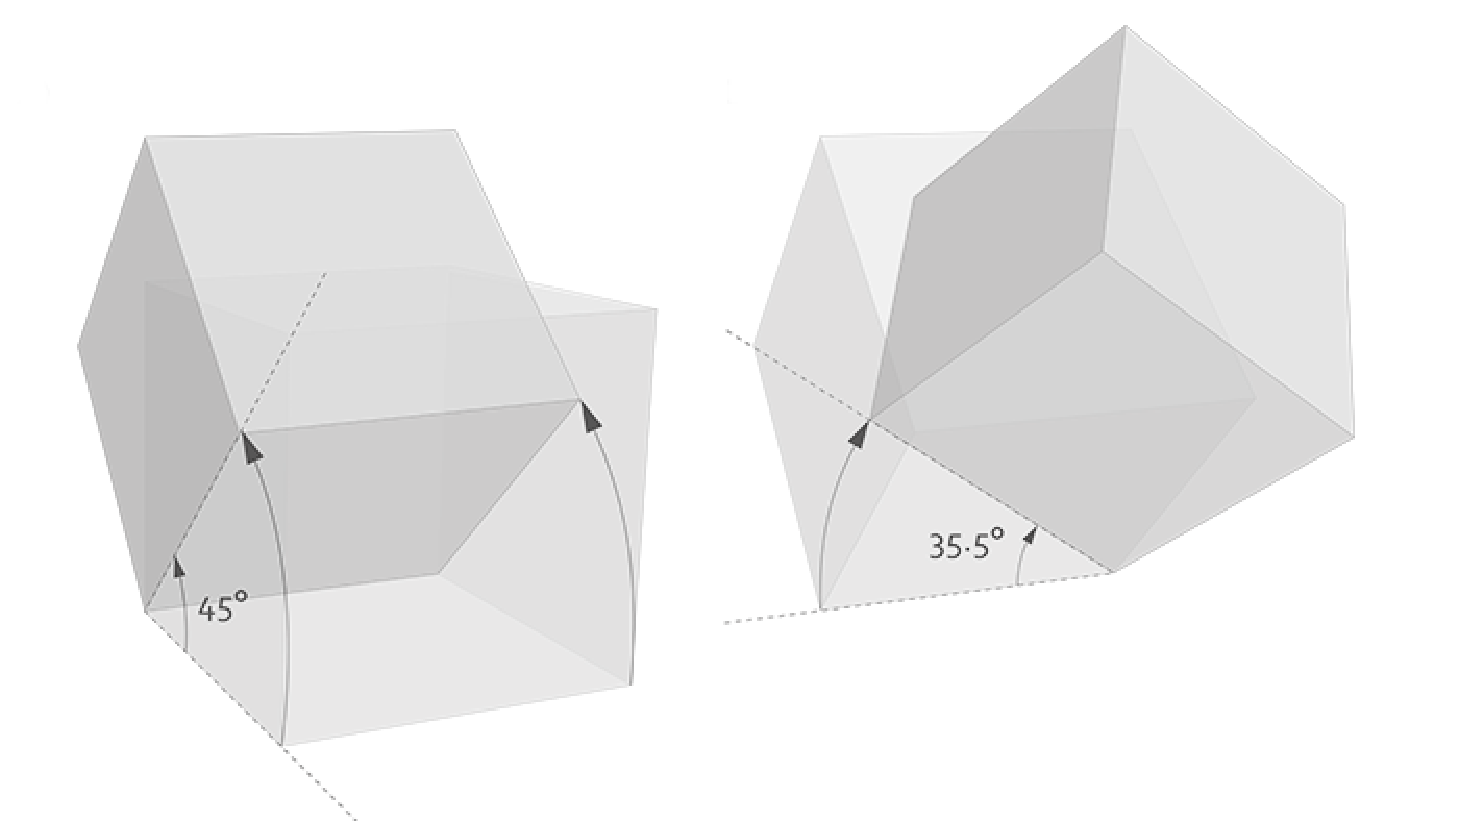
\includegraphics[scale=0.4]{cubli_equilibria}
  \end{center}
  \begin{block}{Upright equilibria (unstable)}
  \[
  \mathcal{E}_{1} = \left\{ \vec{x} \mid \theta_1 \in [-\pi, \pi),\enspace \theta_2 = -\mathrm{atan}\frac{\sqrt{2}}{2},\enspace
   \theta_3 = \frac{\pi}{4},\enspace
    \vec{\dot{\theta}} = \vec{0},\enspace
    \vec{\dot{q}}_{wheels} = \vec{0},\enspace
    \vec{u} = \vec{0}
    \right\}
   \]
  \end{block}
  \begin{block}{Hanging equilibria (stable)}
    \[
    \mathcal{E}_{2} = \left\{
    \vec{x} \mid \theta_1 \in [-\pi, \pi),\enspace
      \theta_2 = \mathrm{atan}\frac{\sqrt{2}}{2},\enspace
    \theta_3 = -\frac{3}{4} \pi,\enspace
    \vec{\dot{\theta}} = \vec{0},\enspace
    \vec{\dot{q}}_{wheels} = \vec{0},\enspace
    \vec{u} = \vec{0}
    \right\}
    \]
  \end{block}
\end{frame}

\section{Controllability}

\begin{frame}{Small time local controllability}
  Given a point $\vec{x}_0$ and an arbitrarily small neighbourhood $V(\vec{x}_0)$ define the set
  \[
  R_{T}^{V}(\vec{x}_0) = \{\vec{x}(\vec{x_0}, T, \bar{\vec{u}}(t)) \mid
  \vec{x}(\vec{x_0}, \tau, \bar{\vec{u}}(t)) \in V(\vec{x}_0) \enspace \forall \tau \in [0,T]\}
  \]
  with $\bar{\vec{u}}$ appropriate inputs
  \par
  A nonlinear system $\dot{\vec{x}} = \vec{f}(\vec{x}, \vec{u})$ is said locally-locally controllable (l.l.c.) from $\vec{x}_0$ if
  \[
  \forall \enspace V(\vec{x}_0) \enspace \exists  \enspace T \enspace
  s.t. \enspace R_{T}^{V}(\vec{x}_0) \enspace \supseteq \enspace B(\vec{x}_0)
  \]
  with $B(\vec{x}_0)$ an open neighbourhood
  \par
  If the time $T$ can be arbitrarily small the system is said small time locally controllable (s.t.l.c.)
\end{frame}

\begin{frame}{s.t.l.c and linear controllability}
  \begin{theorem}
    Consider a nonlinear system $\dot{\vec{x}} = \vec{f}(\vec{x}, \vec{u})$ and an equilibrium point $\vec{x}_{eq}$
    such that $\vec{f}(\vec{x}_{eq}, \vec{0}) = \vec{0}$. If the linear approximation of the system around
    the point $\vec{x}_{eq}$ is completely controllable then the system is small-time locally controllable
    in $\vec{x}_{eq}$.
  \end{theorem}
\end{frame}

\begin{frame}{s.t.l.c and linear controllability (continued)}
  For the system under examination the linear approximation
  \[
  \begin{split}
    \dot{\vec{\delta x}} &= \frac{\partial{\vec{f}(\vec{x},\vec{u})}}{\partial{\vec{x}}}\Big|_{\mathcal{E}_1} \vec{\delta x} +
    \frac{\partial{\vec{f}(\vec{x},\vec{u})}}{\partial{\vec{u}}}\Big|_{\mathcal{E}_1} \vec{\delta u}\\
    &= A \vec{\delta x} + B \vec{\delta u}
  \end{split}
  \]
  is such that the pair $(A, B)$ is not completely controllable. Indeed
  \[
  rank\left(
  \begin{bmatrix}
    B & AB & A^2B & \dots & A^{n-1}B
  \end{bmatrix}
  \right) = 8 < n = 9
  \]
  It is not possible to conclude on the small-time local controllability of the system
  in those points belonging to $\mathcal{E}_1$
\end{frame}

\begin{frame}{Small time local accessibility}
  If $R_{T}^{V}(\vec{x}_0)$ only contains an open set of $\vec{x}_0$
  the small time local controllability becomes small-time local accessibility
  (s.t.l.a).
  \par
  \[
  \Rightarrow
  \]
  \[
  \text{s.t.l.c} \qquad \text{s.t.l.a}
  \]
  \[
  \centernot \Leftarrow
  \]
\end{frame}

\begin{frame}[shrink=10]{Small time local accessibility (continued)}
  Consider a control affine system
  \[
  \dot{\vec{x}} = \vec{f}(\vec{x}) + \sum\limits_{j=1}^{m}\vec{g}_j(\vec{x}) u_{j}
  \]
  and the distributions
  \[
  \mathrm{\Delta}_0 = \mathrm{span} \{\vec{g}_1, \enspace \hdots \enspace, \vec{g}_m\} \quad
  \quad
  \mathrm{\Delta} = \mathrm{span} \{\vec{f},\enspace\vec{g}_1, \enspace \hdots \enspace, \vec{g}_m\}
  \]
  \begin{theorem}
    Consider the smallest $\mathrm{\Delta}$-invariant distribution containing $\mathrm{\Delta}_0$
    called accessibility distribution $<\mathrm{\Delta}|\mathrm{\Delta}_0>$.
    \begin{itemize}
    \item[a.]If the dimension of $<\mathrm{\Delta}|\mathrm{\Delta}_0>= n$ in $\vec{x}_0$ then system
      is s.t.l.a in $\vec{x}_{0}$;
    \item[b.]If $\mathrm{dim}(<\mathrm{\Delta}|\mathrm{\Delta}_0>)= r < n$ in a neighbourhood of $\vec{x}_0$
      then the set $R_{T}^{V}(\vec{x}_0)$ is contained in a submanifold of dimension $r$ of the
      $n$-dimensional state space, and contains an open set in that submanifold.
    \end{itemize}
  \end{theorem}
\end{frame}

\begin{frame}[shrink=10]{Small time local accessibility (continued)}
  In order to evaluate $<\mathrm{\Delta}|\mathrm{\Delta}_0>$ for the system under examination
  the following filtration of distributions
  \[
  \begin{cases}
    \mathrm{\Delta}_1 &= \mathrm{\Delta}_0 + [\mathrm{\Delta}_0,\mathrm{\Delta}]\\
    &\vdotswithin{=} \\
    \mathrm{\Delta}_k &= \mathrm{\Delta}_{k-1} + [\mathrm{\Delta}_{k-1},\mathrm{\Delta}]
  \end{cases}
  \]
  was performed using the Symbolic Math Toolbox from MATLAB until an integer $k$ was found s.t.
  \[
  \text{dim}(\mathrm{\Delta}_{k}(\vec{x}_0)) = \text{dim}(\mathrm{\Delta}_{k+1}(\vec{x}_0))
  \]
  It turns out that for all $\vec{x}_{0} \in \mathcal{E}_{1}$ 
  \[
  \begin{split}
    &k = 3\\
    &\mathrm{dim}(<\mathrm{\Delta}|\mathrm{\Delta}_0>) = 8 < n = 9
  \end{split}
  \]
  Hence $R_{T}^{V}(\mathcal{E}_{1})$ is containted in a submanifold of dimension $8$

\end{frame}

\begin{frame}{Weak local accessibility}
  Although the system is not s.t.l.a in the points of interest it could be local accessible
  in a weaker sense, i.e., without the requirement that the time $T$ is arbitrarily small.
  \par
  A \emph{necessary} condition for weak local accessibility is
  \[
  \mathrm{dim}(<\mathrm{\Delta}|\mathrm{\Delta}>) = n
  \]
  \par
  For the system under examination however
  \[
  \mathrm{dim} <\mathrm{\Delta},\mathrm{\Delta}> = 8 < n = 9
  \quad \forall \vec{x}_0 \in \mathcal{E}_1
  \]
  \alert{The system is not locally accessible in any sense hence it can't be locally controllable}
\end{frame}

\section{Observability}
In this section the nonlinear \emph{local} observability of the system is discussed.
The concept of local observability can be explained in terms of the indistinguishability
between a given \emph{initial} state $\bar{\vec{x}}$ and another initial state ``near'' $\bar{\vec{x}}$ namely
$\bar{\vec{x}} + \vec{\delta x}$.
\par
The initial states $\bar{\vec{x}}$ and $\bar{\vec{x}} + \vec{\delta x}$ are said to be
indistinguishable in the interval $[0, T]$ if for every input $\vec{u}$ the outputs
$\vec{y(\bar{\vec{x}}, \vec{u}, t)} = \vec{y(\bar{\vec{x}} + \vec{\delta x}, \vec{u}, t)}$
for every $t \in [0, T]$.
\par
Local indistinguishability can be assessed using appropriate tools from the theory
of nonlinear systems and in some cases using the theory of LTI systems as explained
in the following.

\subsection{Linear Observability}
In order to study the local indistinguishability between two initial states using the theory of LTI systems
the following theorem can be used.
\begin{theorem}
  Consider a nonlinear system 
  \[
  \begin{cases}
    \dot{\vec{x}} = \vec{f}(\vec{x}, \vec{u})\\
    \vec{y} = \vec{h}(\vec{x}, \vec{u})
  \end{cases}
  \]
  and an equilibrium point $\vec{x}_{eq}$ such that $\vec{f}(\vec{x}_{eq}, \vec{0}) = \vec{0}$.
  If the linear approximation of the system around the point $\vec{x}_{eq}$ is completely
  observable then there are no indistinguishable points from $\vec{x}_{eq}$ in a small enough
  neighbourhood of $\vec{x}_{eq}$.
\end{theorem}
It is recalled that a linear system
\[
\dot{\vec{\delta x}} = A \vec{\delta x} + B \vec{\delta u}
\]
\[
\dot{\vec{\delta y}} = C \vec{\delta x}
\]
where
\[
\vec{\delta x}(t) = \vec{x}(t) - \vec{x}_{eq} \quad \vec{\delta u}(t) = \vec{u}(t) - \vec{u}_{eq} \quad
\vec{\delta y}(t) = \vec{y}(t) - \vec{h}(\vec{x}_{eq}, \vec{u}_{eq})
\]
is observable if the rank of the observability matrix $R_o$ 
\begin{equation} \label{eq:linear_observability}
R_o = 
\begin{bmatrix}
C \\ CA \\ CA^2 \\ \vdots \\ CA^{n-1}
\end{bmatrix}
\end{equation}
is equal to the dimension of the state $n$.
\par
For the system of equations (\ref{eq:nl_eq_2}) and (\ref{eq:output}) it can be found that the linear approximation
around each equilibrium point belonging to $\mathcal{E}_{1}$ is not completely observable and
the matrix $R_o$ has rank $6 < n = 9$. As a consequence it is not possible to conclude on
the local indistinguishability relative to those points.

\subsection{Nonlinear Observability}
As done for the nonlinear local controllability the definition of local
indistinguishability should be refined with the requirement that
the inputs $\vec{u}$ are such that the state trajectory never goes outside of
a neighbourhood of the initial states for every $t \in [0, T]$.
The notation used to denote two indistinguishable initial states $\bar{\vec{x}}_1$
and $\bar{\vec{x}}_2$ in the interval $[0,T]$ is
\[
\bar{\vec{x}}_1 I^{U}_{T} \bar{\vec{x}}_2
\]
where $U \subseteq \{\vec{u}(\cdot):[0,T] \rightarrow \mathbb{R}^{m}\}$ contains
input functions which satisfy the hypothesis given above.
\par
In order to study the nonlinear locally indistinguishability of a system written in control affine form
\begin{equation}\label{eq:nonlinear_system_outputs}
  \begin{cases}
    \dot{\vec{x}} = \vec{f}(\vec{x}) + g(\vec{x}) \vec{u}\\
    \vec{y} = \vec{h}(\vec{x}, \vec{u})
  \end{cases}
\end{equation}
the codistribution
\[
\mathrm{\Omega}_0 = \mathrm{span} \{ d \vec{h}\}
\]
and the distribution
\[
\mathrm{\Delta}= \mathrm{span} \{\vec{f},\enspace\vec{g}_1, \enspace \hdots \enspace, \vec{g}_m\}
\]
have to be considered. The following theorem holds
\begin{theorem}\label{th:obs}
  Consider the smallest $\mathrm{\Delta}$-invariant codistribution containing $\mathrm{\Omega}_0$ called
  observability codistribution $< \mathrm{\Delta} | d\vec{h} >$.
  \begin{itemize}
  \item[a.]If the dimension of $< \mathrm{\Delta}|d\vec{h} >$ is equal to $n$ in $\bar{\vec{x}}$ then
    there are no initial states ``near'' $\bar{\vec{x}}$ that are indistinguishable from
    it and the system (\ref{eq:nonlinear_system_outputs}) is said locally observable in $\bar{\vec{x}}$;
  \item[b.]If $\text{dim}(< \Delta|\Omega_0 >) = d < n$ in a neighbourhood of $\bar{\vec{x}}$ then
    the $(n-d)$-dimensional distribution $< \Delta|\Omega_0 >^{\perp}$ that annihilates
    the observability codistribution is involutive. Clearly such distribution evaluated at $\bar{\vec{x}}$
    identifies the displacements $\vec{\delta{x}}$ such that $\bar{\vec{x}} I^{U}_{T}(\bar{\vec{x}} + \vec{\delta x})$
  \end{itemize}
\end{theorem}
\par
In order to evaluate the observability codistribution for the system under examination
(equations \ref{eq:nl_eq_2} and \ref{eq:output}) the following filtration of codistributions
\[
\begin{cases}
\Omega_1 &= \Omega_0 + L_\Delta \Omega_0\\
&\vdotswithin{=} \\
\Omega_k &= \Omega_{k-1} + L_\Delta \Omega_{k-1}
\end{cases}
\]
was performed until an integer $k$ was found such that
\[
\mathrm{dim}(\Delta_{k}(\bar{\vec{x}})) = \mathrm{dim}(\Delta_{k + 1}(\bar{\vec{x}}))
\]
\par
It turns out that for all $\bar{\vec{x}} \in \mathcal{E}_{1}$, i.e.,the cubic frame
is standing still in the upright configuration with zero flywheel velocities,
\[
\mathrm{dim} (<\mathrm{\Delta},d\vec{h}>) = 6 < n = 9
\]
but the codistribution is not regular, i.e., the dimension is not constant in a neighbourhood
of a given $\bar{\vec{x}} \in \mathcal{E}_{1}$ hence the theorem (\ref{th:obs}) cannot be applied.
Conversely any given initial state in which the cubic frame is standing still in the upright
configuration with \emph{non zero angular rates} gives
\[
\mathrm{dim} (<\mathrm{\Delta},d\vec{h}>) = n
\]
hence the system is locally observable in those points.
\newpage

\section{Noninteracting controller}

\begin{frame}[shrink=10]{Theory of Noniteracting control}
  Consider a nonlinear control affine system with $m$ inputs and $m$ outputs
  \[
  \vec{\dot{x}} = \vec{f}(\vec{x}) + \sum\limits_{i=1}^{\alert{m}} \vec{g}_{i}(\vec{x}) u_{i}
  \]
  \[
  y_{1} = h_{1}(\vec{x})
  \]
  \[
  \hdots
  \]
  \[
  y_{m} = h_{\alert{m}}(\vec{x})
  \]
  and an initial point $\vec{x}^{0}$
  \par
  The problem of noninteracting control is stated as finding a regular static state feedback
  \[
  \vec{u}(\vec{x})  = \vec{\alpha}(\vec{x}) + \vec{\beta}(\vec{x}) \vec{v} \quad \vec{x} \in B_{\delta}(\vec{x}^0)
  \]
  such that in the resulting closed loop system each output $y_i$ is affected
  only by the corresponding input $v_i$ and not by the others.
\end{frame}

\begin{frame}{Theory of Noniteracting control (continued)}
  Suppose that the system has a vector relative degree $\{r_1, \hdots, r_m\}$ at $\vec{x}^{0}$ hence it admits
  a \emph{normal form} locally around $\vec{x}^{0}$
  \begin{columns}[t]
    \begin{column}{0.5\textwidth}
      \[
      \dot{\xi}_{1}^{i} = \xi_{2}^{i}
      \]
      \[
      \hdots
      \]
      \[
      \dot{\xi}_{r_{i}-1}^{i} = \xi_{r_{i}}^{i}
      \]
      \[
      1 \le i \le m
      \]
      \[
      \begin{bmatrix}
        \dot{\xi}_{r_{1}}^{1}\\
        \vdots\\
        \dot{\xi}_{r_{m}}^{m}\\
      \end{bmatrix}=
      \vec{b}(\vec{\xi},\vec{\eta}) + A(\vec{\xi},\vec{\eta})\vec{u}
      \]
    \end{column}
    \begin{column}{0.5\textwidth}
      \[
      \vec{\dot{\eta}} = \vec{q}(\vec{\xi},\vec{\eta}) + \vec{p}(\vec{\xi},\vec{\eta})\vec{u}
      \]
      \vskip0.3in
      \[
      \begin{bmatrix}
        \vec{\xi}\\
        \vec{\eta}
      \end{bmatrix} = 
      \Phi(\vec{x})
      \]
    \end{column}
  \end{columns}
  \centering
  with $A(\vec{x})$ nonsingular at $\vec{x}^{0}$
\end{frame}

\begin{frame}{Theory of Noniteracting control (continued)}
  \begin{block}{Proposition (Isidori)}
    Suppose
    \[
    L{\vec{g}_j}L_{\vec{f}}^{k}h_{i}(\vec{x}) = 0 \enspace \forall \vec{x} \in B_{\delta}(\vec{x}^0)
    \]
    \[
    1 \le j \le m, \enspace 1 \le i \le m, \enspace k < r_i-1
    \]
    and
    \[
    \begin{bmatrix}
      L_{\vec{g}_1}L_{\vec{f}}^{r_{i-1}}h_i(\vec{x}^{0}) \enspace \hdots \enspace L_{\vec{g}_m}L_{\vec{f}}^{r_i-1}h_i(\vec{x}^{0})
    \end{bmatrix}
    \ne
    \begin{bmatrix}
      0 \enspace \hdots \enspace 0
    \end{bmatrix}
    \enspace 1 \le i \le m
    \]
    Then the noninteracting control problem is solvable iff the matrix $A(\vec{x}^{0})$ is nonsingular,
    i.e. if the system has a vector relative degree $\{r_1, \hdots, r_m\}$ at $\vec{x}^{0}$
  \end{block}
\end{frame}

\begin{frame}{Theory of Noniteracting control (continued)}
  Indeed the regular static feedback
  \[
  \vec{u} = -A^{-1}(\vec{\xi},\vec{\eta})\vec{b}(\vec{\xi},\vec{\eta}) + A^{-1}(\vec{\xi},\vec{\eta})\vec{v}
  \]
  results in the closed loop system
  \begin{columns}[t]
    \begin{column}{0.5\textwidth}
      \[
      \dot{\xi}_{1}^{i} = \xi_{2}^{i}
      \]
      \[
      \hdots
      \]
      \[
      \dot{\xi}_{r_{i}-1}^{i} = \xi_{r_{i}}^{i}
      \]
      \[
      \dot{\xi}_{r_{i}}^{i} = v_{i}
      \]
      \[
      y_{i} = \xi_{1}^{i}
      \]
      \[
      1 \le i \le m
      \]
    \end{column}
    \begin{column}{0.5\textwidth}
      \[
      \vec{\dot{\eta}}  = \hat{\vec{q}}(\vec{\xi},\vec{\eta}) + \hat{\vec{p}}(\vec{\xi},\vec{\eta})\vec{v}
      \]
    \end{column}
  \end{columns}
\end{frame}

\begin{frame}{Application of the Noniteracting control}
  For the system under examination
  \[
  \begin{cases}
    \begin{split}
      \dot{\vec{x}} &= \vec{f}(\vec{x}) + g(\vec{x})\vec{u}\\
      &=\vec{f}(\vec{x}) +
      \begin{bmatrix}
        0_{3\times3} \\
        \left(B(\theta_2,\theta_3) ^ {-1}\right)_{(:, 4:6)}
      \end{bmatrix}\vec{u}\\
    \end{split}\\
    \vec{y} = \vec{h}(\vec{x}) =
    \begin{bmatrix}
      \theta_1 &
      \theta_2 &
      \theta_3
    \end{bmatrix} \transpose
  \end{cases}
  \]
  it can be found that
  \[
  L_{\vec{g}_{j}}L_{\vec{f}}^{0}h_{i} =
  L_{\vec{g}_{j}}h_{i} = 
  \begin{bmatrix}
    \vec{e}_i & 0_{6x1}
  \end{bmatrix}
  \vec{g}_j
  =
  g_{j}^{i} = 0
  \qquad 1 \le j \le 3, \enspace 1 \le i \le 3
  \]

\end{frame}

\begin{frame}{Existence of a vector relative degree}
  Also 
  \[
  \frac{\mathrm{d}^{2}}{\mathrm{d}t^{2}}\vec{y} = 
  \begin{bmatrix}
    \ddot{\theta_1}\\
    \ddot{\theta_2}\\
    \ddot{\theta_3}
  \end{bmatrix} =
  \vec{b}(\vec{x}) + A(\vec{x}) \vec{u}
  \]
  where
  \[
  \vec{b}(\vec{x}) = \vec{f}(\vec{x})_{(4:6)}
  \]
  and
  \[
  A(\vec{x}) = \left(B(\theta_2,\theta_3) ^ {-1}\right)_{(1:3, 4:6)}
  \]
\end{frame}

\begin{frame}{Existence of a vector relative degree (continued)}
  \centering
  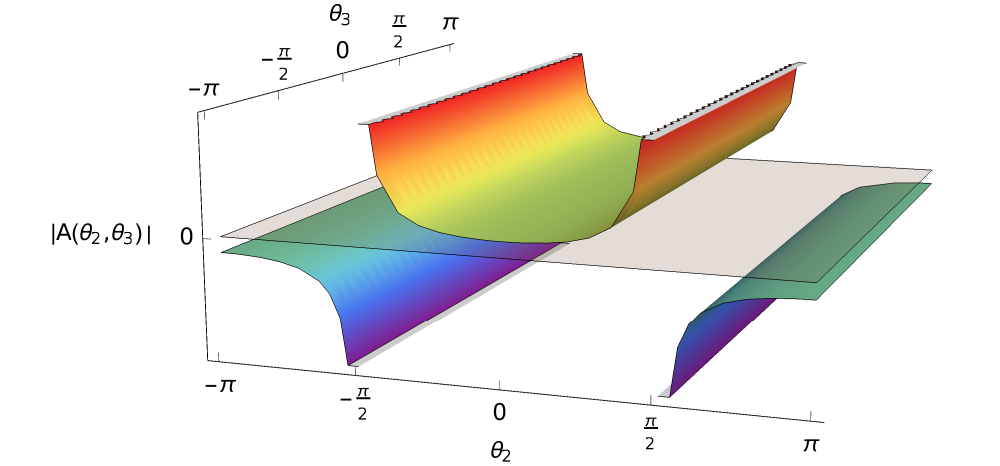
\includegraphics[scale=0.4]{detA.png}
  \[
  |A| \ne 0 \enspace \forall \theta_2, \theta_3 \implies \{r_1, r_2, r_3\} = \{2,2,2\} \enspace \forall \vec{x}
  \]
  The resulting standard noninteractive feedback is
  \[
  \vec{u}_{NIC} = -\left(B(\theta_2,\theta_3) ^ {-1}\right)_{(1:3, 4:6)}^{-1}
  (\vec{f}_{(4:6)}(\vec{x}) - \vec{v} )
  \]
\end{frame}

\begin{frame}[shrink=10]{Unobservable part of the system}
  The unobservable part of the system can be obtained by completely specifying
  the coordinate transformation $\Phi$
  \[
  \vec{y} =
  \begin{bmatrix}
    \theta_1 &
    \theta_2 &
    \theta_3
  \end{bmatrix}\transpose
  \implies
  \Phi(\vec{x})_{1:6} =
  \begin{bmatrix}
    \theta_1 & \dot{\theta}_1 &  \theta_2 & \dot{\theta}_2 &
    \theta_3 & \dot{\theta}_3
  \end{bmatrix}\transpose
  \]
  The remaining part is chosen as
  \[
  \Phi(\vec{x})_{1:6} =
  \begin{bmatrix}
    \dot{q}_x & \dot{q}_y & \dot{q}_z
  \end{bmatrix}\transpose
  \]
  i.e. the unobservable part of the closed loop system is the closed loop dynamics of the
  flywheels
  \[
  \begin{split}
    \dot{\vec{\eta}} &=
    \begin{bmatrix}
      \ddot{q}_{x}\\
      \ddot{q}_{y}\\
      \ddot{q}_{z}
    \end{bmatrix}
    = \vec{f}_{(7:9)}(\vec{x}) + \left(B(\theta_2,\theta_3) ^ {-1}\right)_{(4:6, 4:6)} \vec{u}_{NIC}\\
    &=\vec{f}_{(7:9)}(\vec{x}) - \left(B(\theta_2,\theta_3) ^ {-1}\right)_{(4:6, 4:6)}
    \left(B(\theta_2,\theta_3) ^ {-1}\right)_{(1:3, 4:6)}^{-1}
    (\vec{f}_{(4:6)}(\vec{x}) - \vec{v})\\
    &=\hat{\vec{q}}(\vec{x}) + \hat{\vec{p}}(\theta_{2},\theta_{3})\vec{v}
  \end{split}
  \]
\end{frame}

\begin{frame}{Yaw motion while balancing on a corner}
  Consider a rotation about the $z$ axis of the inertial
  reference frame $\{S\}$ while the balance on one of the corner is maintained
  \begin{center}
    \includemedia[
      activate=pageopen,
      width=200pt,height=200pt,
      addresource=videos/cubli_yaw_noerr.mp4,
      flashvars={%
        src=videos/cubli_yaw_noerr.mp4
        &scaleMode=stretch&autoPlay=true&loop=true
        &hideBar=true}
    ]{}{StrobeMediaPlayback.swf}
  \end{center}
\end{frame}

\begin{frame}{Yaw motion while balancing on a corner (continued)}
  A suitable control law $\vec{v}$ is
  {\small
    \[
    \begin{split}
      &v_1(t) = \ddot{\theta}_1^{des}(t) + k_d(\dot{\theta}_1^{des}(t) - \dot{\theta}_1(t)) + k_p (\theta_1^{des}(t) - \theta_1(t))\\
      &v_2(t) = - k_d\dot{\theta}_2(t) + k_p \left(-\mathrm{atan}\frac{\sqrt{2}}{2} - \theta_2(t)\right)\\
      &v_3(t) = - k_d\dot{\theta}_3(t) + k_p \left(\frac{\pi}{4} - \theta_3(t)\right)
    \end{split}
    \]
  }
  where
  \[
  \theta_1^{des}(t) = a_0 + a_1 t + a_2 t^2 + a_3 t^3 + a_4 t^4 + a_5 t^5
  \]
  with boundary conditions
  \[
  \begin{split}
    &\theta_1^{des}(0) \in [-\pi, \pi) \quad \dot{\theta}_1^{des}(0)= 0 \quad \ddot{\theta}_1^{des}(0) = 0\\
      &\theta_1^{des}(t_{f}) \in [-\pi, \pi)  \quad \dot{\theta}_1^{des}(t_{f})= 0 \quad \ddot{\theta}_1^{des}(t_{f}) = 0
  \end{split}
  \]
\end{frame}

\begin{frame}{Results}
  \[\theta_1^{des}(0) = \SI{0}{\degree} \rightarrow \theta_1^{des}(2) = \SI{100}{\degree}
  \rightarrow \theta_1^{des}(4) = \SI{0}{\degree}\]
  \[k_p = 10 \enspace k_d = 0.1\]
  \begin{center}
    \includemedia[
      activate=pageopen,
      width=288pt,height=162pt,
      addresource=videos/cubli_yaw_youtube.mp4,
      flashvars={%
        src=videos/cubli_yaw_youtube.mp4
        &scaleMode=stretch&autoPlay=true}
    ]{}{StrobeMediaPlayback.swf}
  \end{center}
\end{frame}

\begin{frame}{Results (continued)}
  The flywheel velocities $\vec{\eta}(t)$ which are
  solution to the differential equation
  \[
  \begin{cases}
    \dot{\vec{\eta}} = \hat{\vec{q}}(\vec{x}) + \hat{\vec{p}}\left(-\mathrm{atan}\frac{\sqrt{2}}{2},\frac{\pi}{4}\right)\vec{v}_{PD}\\
    \vec{\eta}(0) = \vec{0}
  \end{cases}
  \]
  are bounded and tends to zero
  \par
  \centering
  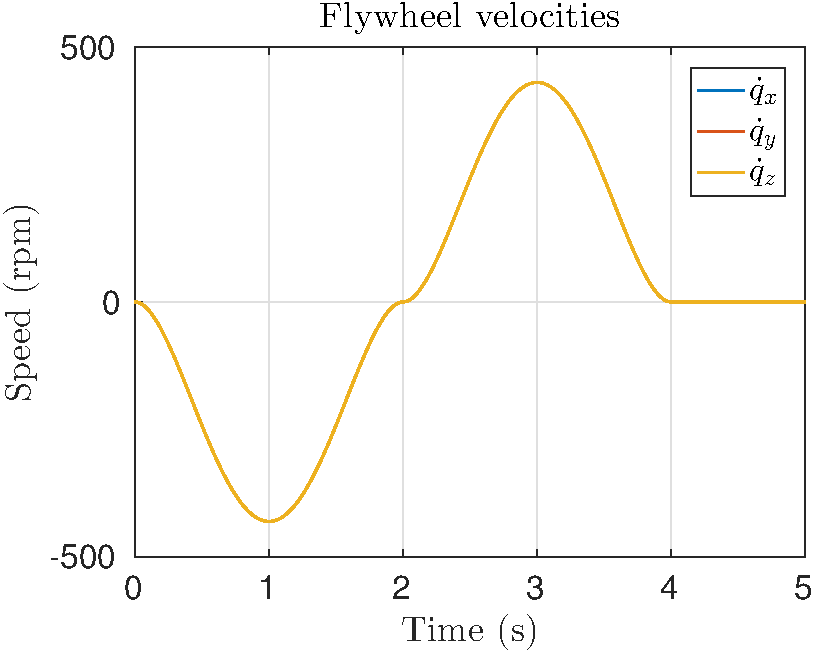
\includegraphics[scale=0.4]{fly_wheel2}
\end{frame}

\begin{frame}{Use of an alternative Euler parametrization}
  Using a different parametrization of the rotation matrix
  \[
  R_{SC}(\vec{\theta}) = R_x(\theta_1)R_y(\theta_2)R_z(\theta_3)
  \]
  the same results apply but the desired yaw motion requires to specify
  all three angles using Slerp.
  \par
  However in this setup the unobservable part of the closed loop system, i.e.
  the flywheels velocities, does not tend to zero. A possible solution is to switch
  to a LQR based control after the rotation is completed to slow down the flywheels.
  \par
  This approach works if the flywheels velocities before the switch are not too high.
\end{frame}

\begin{frame}{Results}
  \vskip0.1in
  \begin{columns}
    \begin{column}{0.45\textwidth}
      \begin{itemize}
      \item[-]$k_p = 2500$, $k_d = 50$
      \item[-]rotation of $\SI{180}{\degree}$ in $\SI{4}{\second}$
      \item[-]LQR control actived at $t = \SI{5}{\second}$ 
      \end{itemize}
    \end{column}
    \begin{column}{0.45\textwidth}
      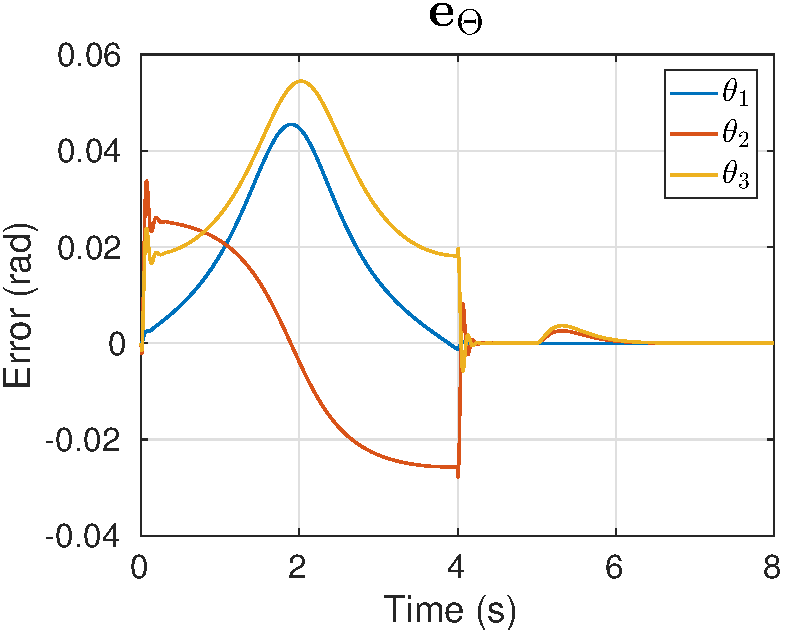
\includegraphics[width=\columnwidth]{error_lqr}
    \end{column}
  \end{columns}
  \begin{columns}
    \begin{column}{0.45\textwidth}
      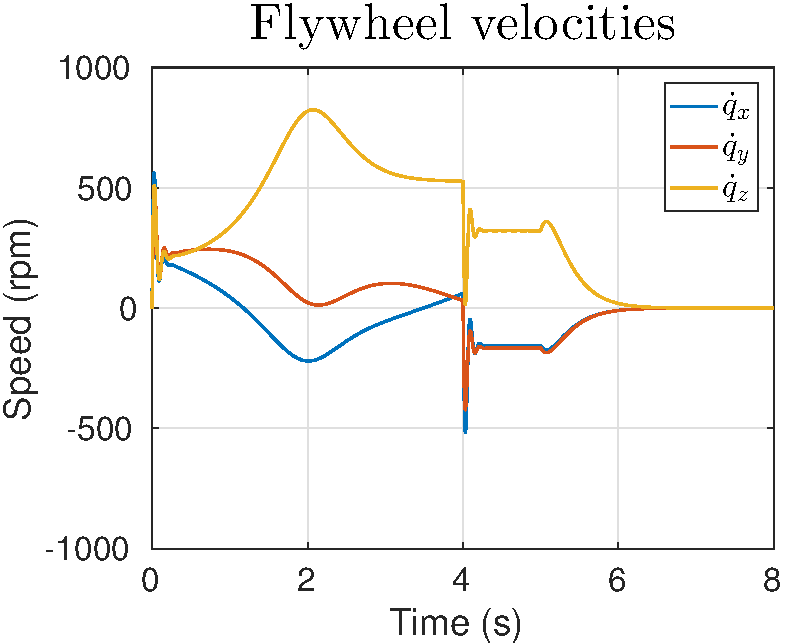
\includegraphics[width=\columnwidth]{fly_wheel_lqr}
    \end{column}
    \begin{column}{0.45\textwidth}
      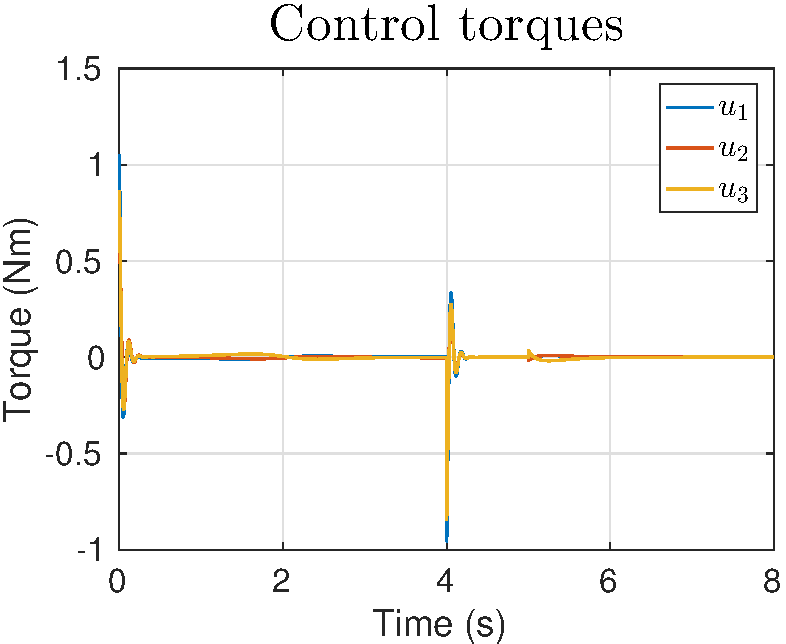
\includegraphics[width=\columnwidth]{input_lqr}
    \end{column}
  \end{columns}
\end{frame}

%% \begin{frame}{Results ($k_p = 2500$, $k_d = 50$)}
%%   \centering
%%   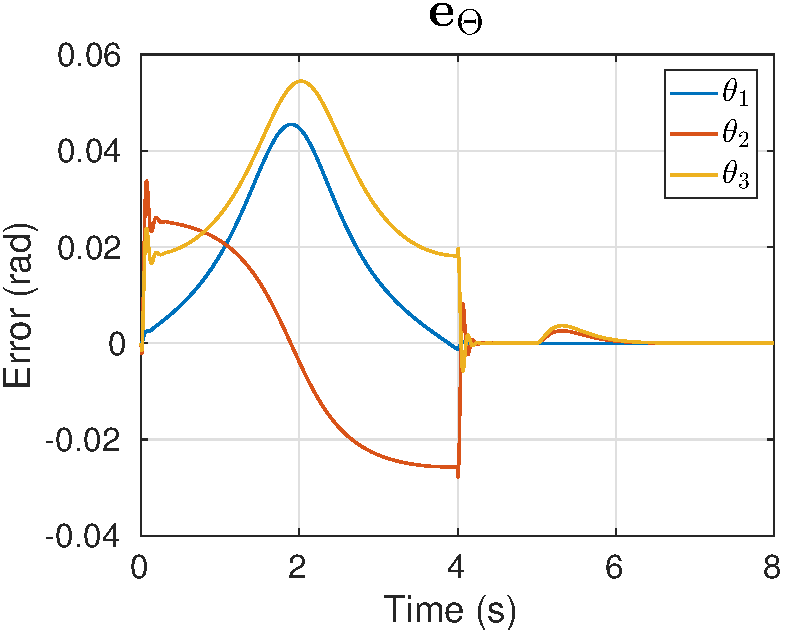
\includegraphics[scale=0.4]{error_lqr}
%%   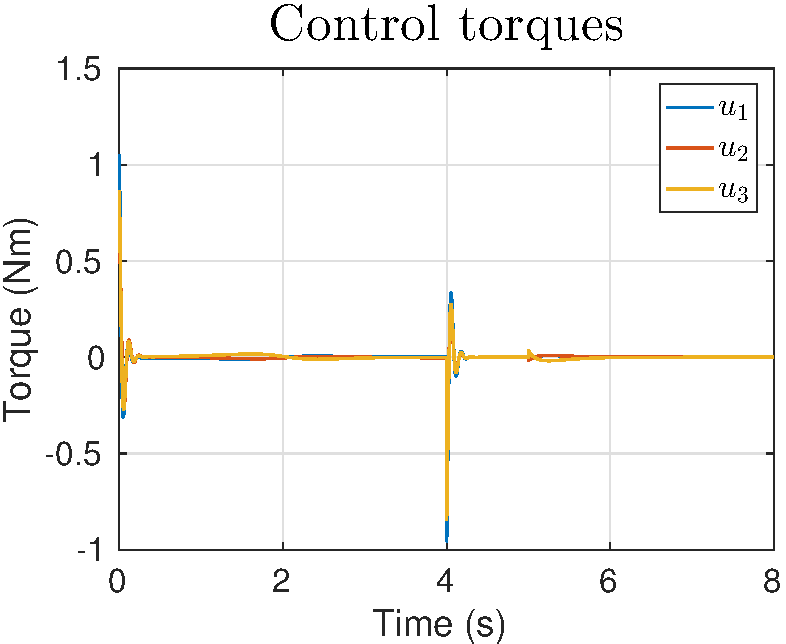
\includegraphics[scale=0.4]{input_lqr}
%% \end{frame}

%% \begin{frame}{Results}
%%   The LQR control is actived at $t = \SI{5}{\second}$
%%   \par
%%   \centering
%%   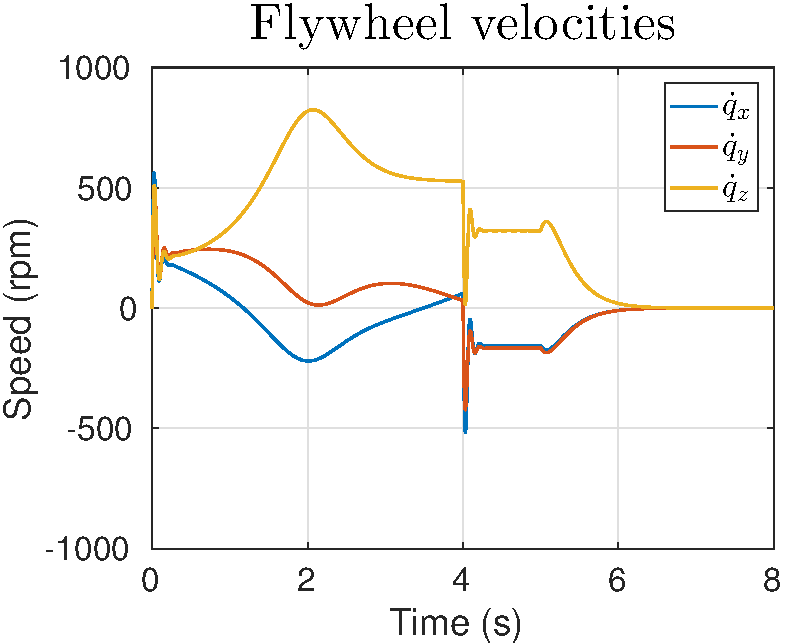
\includegraphics[scale=0.6]{fly_wheel_lqr}
%% \end{frame}

\begin{frame}{Results}
  The outcome of the switch to the LQR controller
  is shown for several angles of rotation and several durations of the movement
  \par
  \centering
  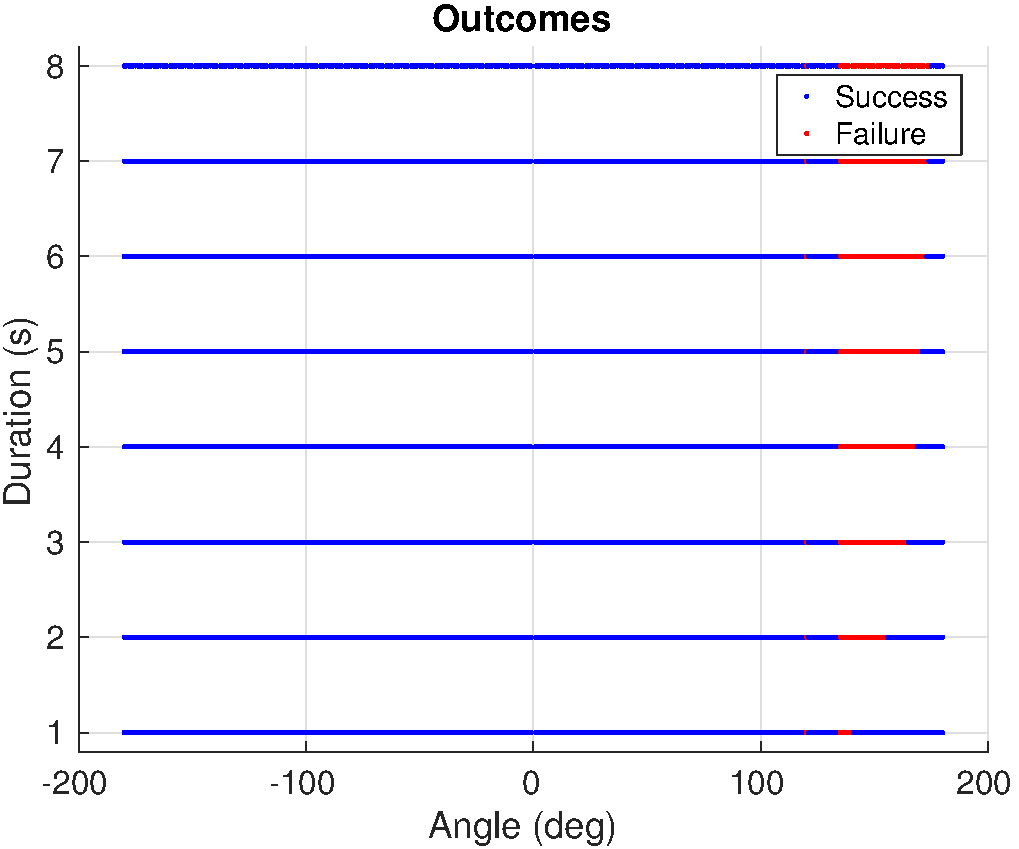
\includegraphics[scale=0.46]{simulation_lqr}
\end{frame}

\begin{frame}{Results}
  The failures happen when the flywheel velocities are too high as expected
  \par
  \centering
  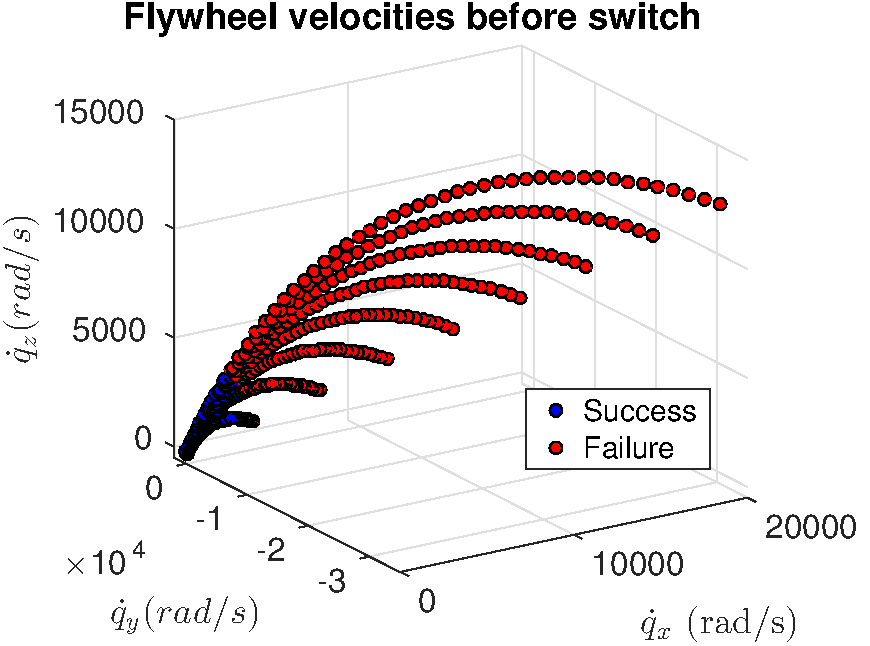
\includegraphics[scale=0.62]{simulation_lqr_velocities}
\end{frame}



\end{document}
